\documentclass[t]{beamer}

%% ----------------------------------------------------- PACKAGES ----------------------------------------------------- %%
\usepackage{coolPrez}
\usepackage{tikz}
\bibliography{bibfile.bib}
%% ---------------------------------------------------- DOCUMENT ---------------------------------------------------- %%

\begin{document}

%% TITLE PAGE
\title[Learning from largely suboptimal teachers - a compliance approach]{Learning from largely suboptimal teachers and the role of compliance}
\author[]{Louis Faury\\ \vspace{5pt} \small{\textcolor{gray}{Advisors} : Mahdi Khoramshahi \& Andrew Sutcliffe}}
\institute[Semester Project at LASA]{Semester Project at LASA}
\titlegraphic{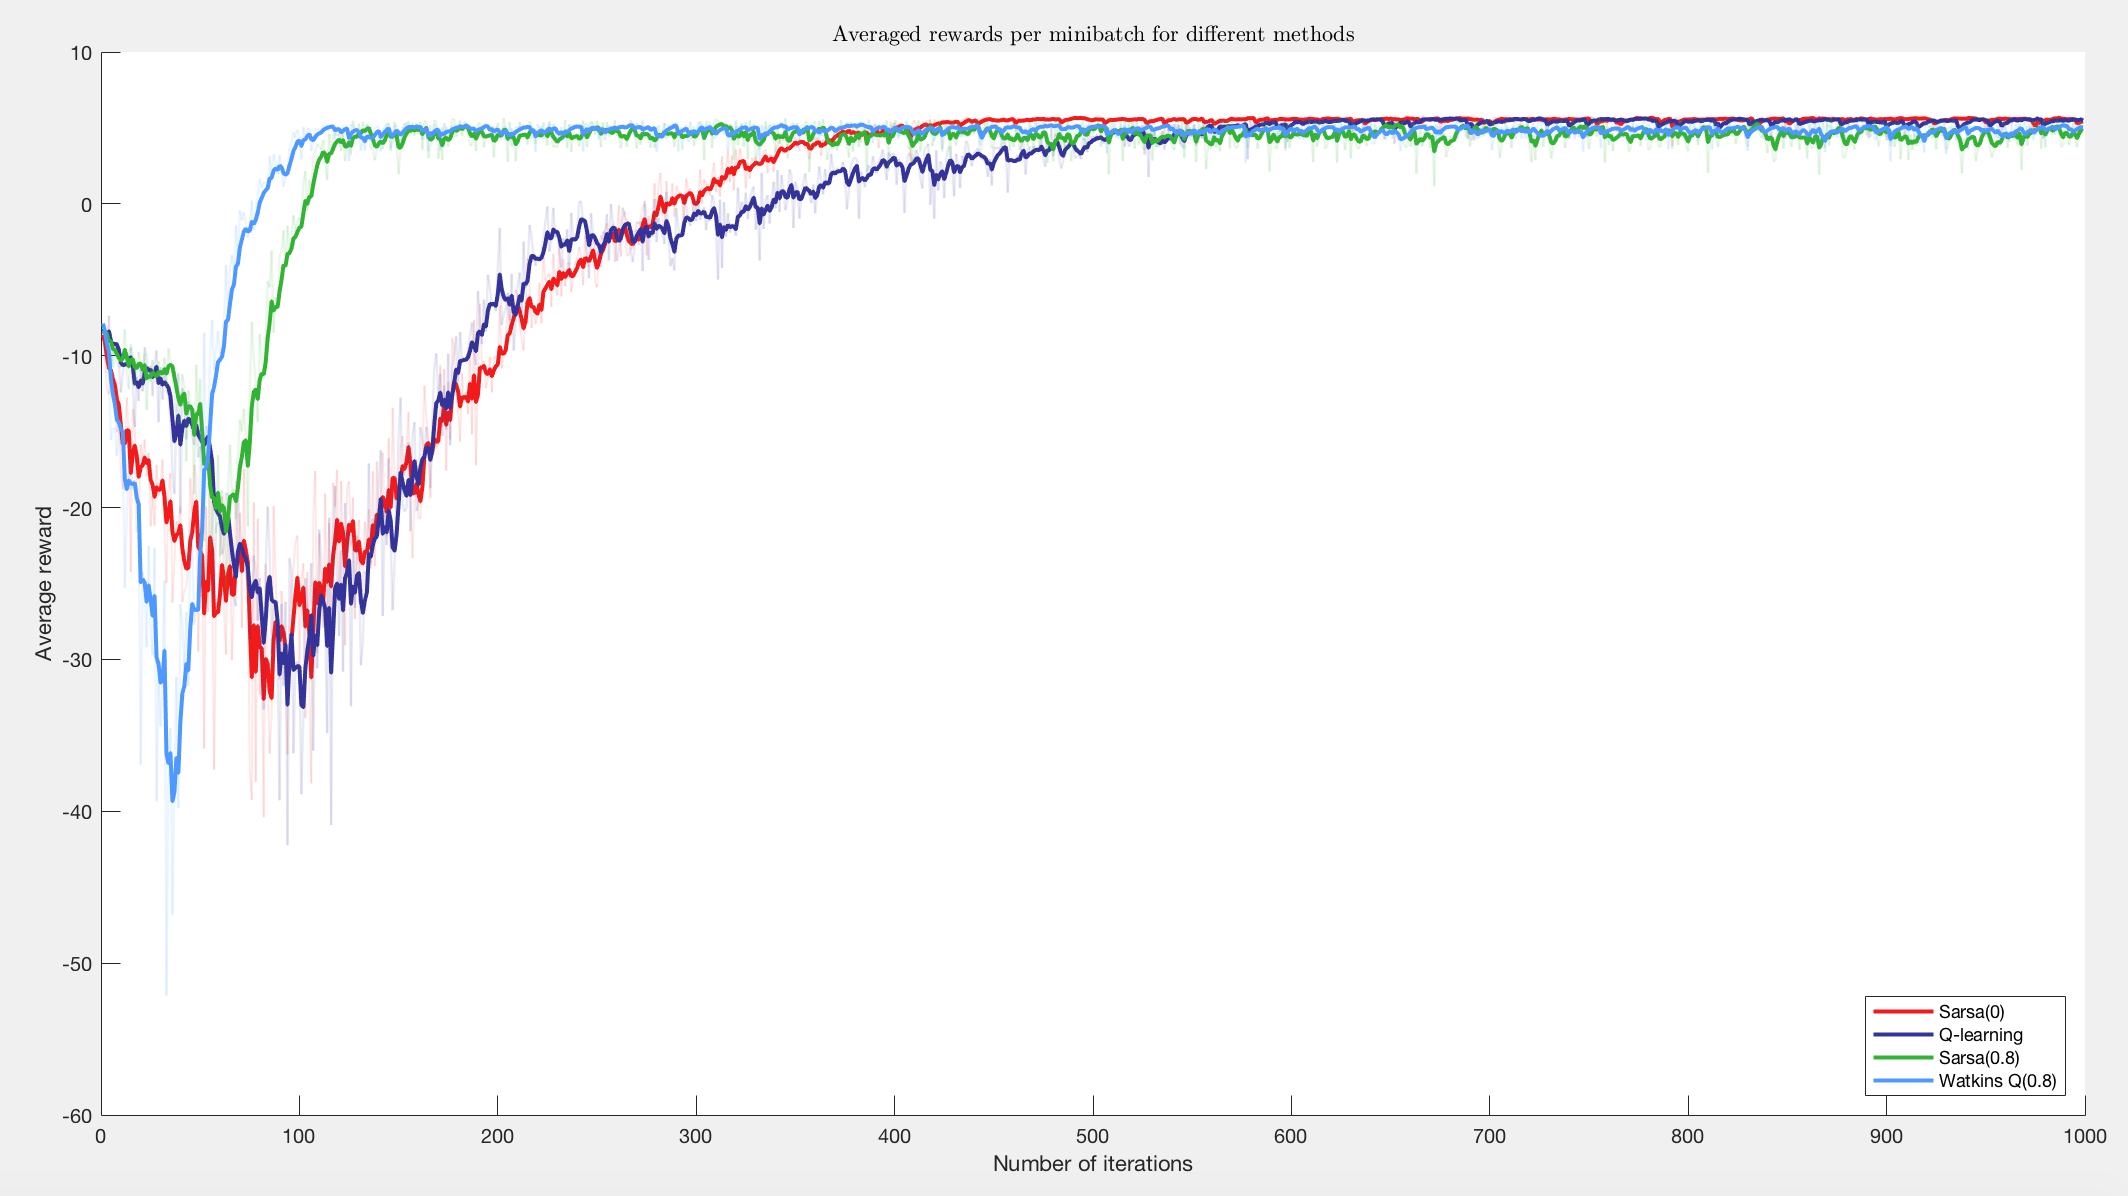
\includegraphics[width=0.7\linewidth]{titlepage_pic}}
\newenvironment{subenv}{\only{\setbeamercolor{local structure}{fg=red}}}{}
\graphicspath{{../report/Images/}}
\titlepage

%1
\begin{frame}[t]
	\vspace{-3ex}
	\frametitle{Plan}
  	\tableofcontents
\end{frame}

\section{Motivations}
{
	\frame[t]
	{
		$\blacksquare$ An example : 
		\begin{center}
			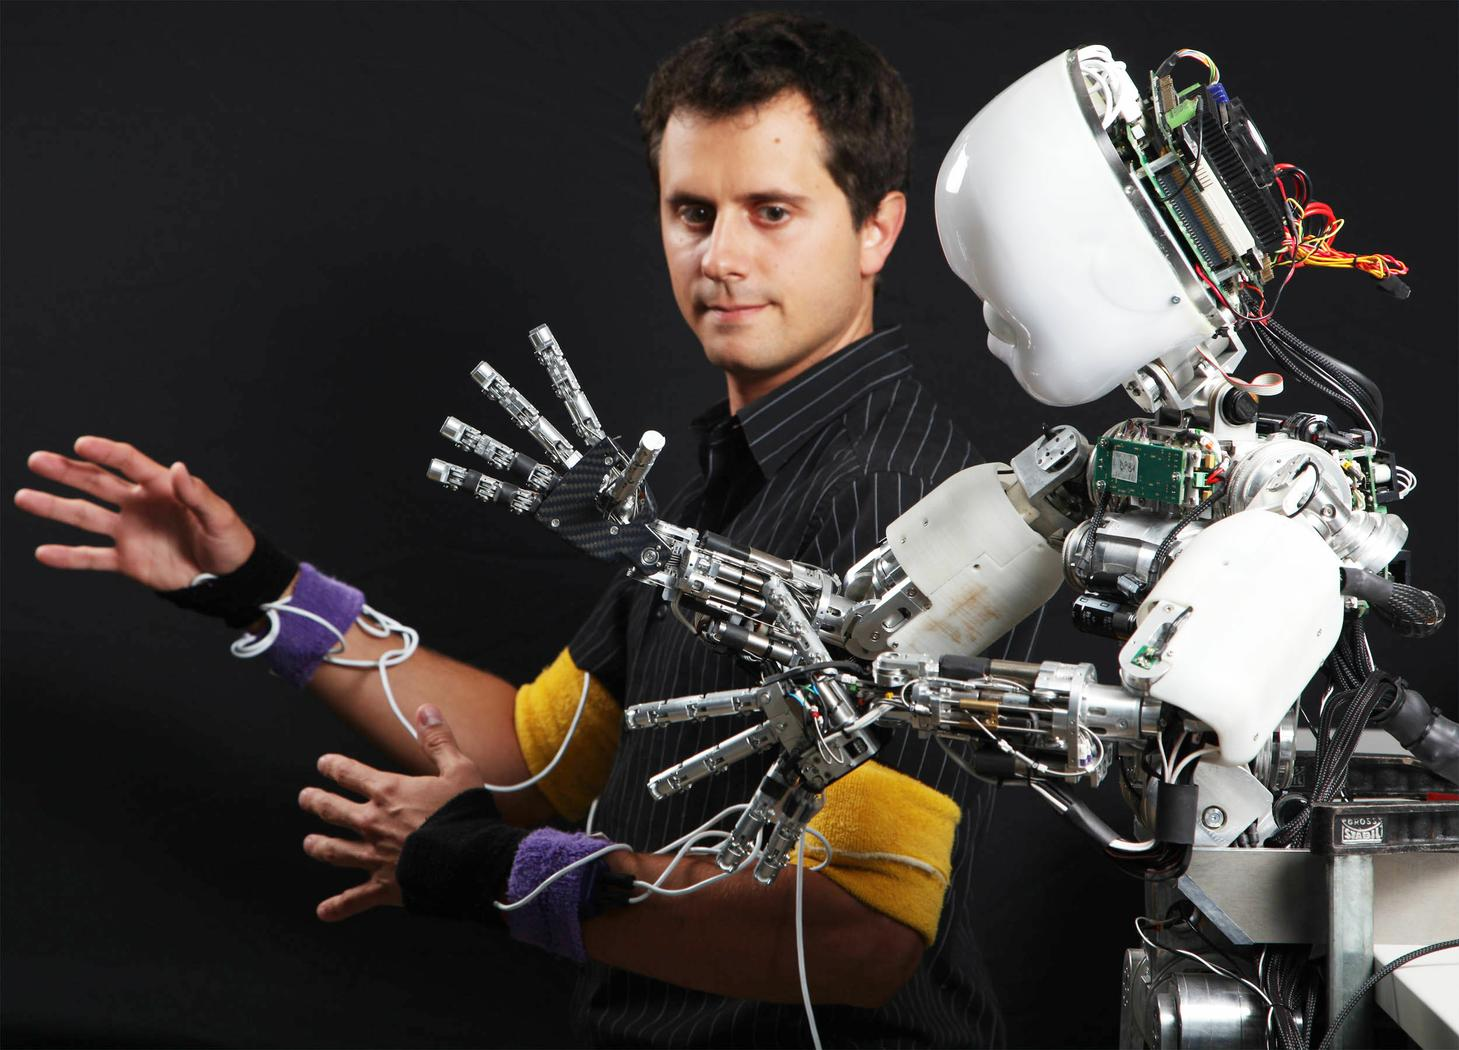
\includegraphics[width=0.7\linewidth]{rob_dem}
		\end{center}
		\vspace{10pt}
		
		\small \emph{Credits} : Sylvain Calinon
	}
	
	\frame[t]
	{
		\vspace{20pt}
		\begin{itemize}
			\item How to take the teacher's demonstration into account?
				\begin{itemize}
					\item<sub@1> Exactly reproduce the teacher's actions 
					\item<sub@1> Use demonstration data to build a representation of the environment's dynamics
					\item<sub@1> \textbf{Use the teacher's demonstration as an exploration baseline}
				\end{itemize}				
		\end{itemize}
		\vspace{20pt}
		\begin{itemize}
			\item Child learning to dance : first follows its teacher's moves, before trying out new ones once he feels he has exploited the teacher's recommandations.
		\end{itemize}
		\hspace{50pt} $\color{red}\Rightarrow$ notion of \textcolor{red}{\textbf{compliance}} w.r.t the teacher. 
	}
	
		\frame[t]
	{
		\vspace{20pt}
		$\small\blacksquare$ \textbf{Goal} : 
			\begin{itemize}
				\item Introduce a theoretical framework for compliance-based learning 
				\item Grasp ideas and intuitions about how such an approach can 
				\begin{itemize}
					\item<sub@1> Overcome a mentor's (large) sub-optimality. 								\item<sub@1> Speed up the learning   
					\item<sub@1> Generalize to \emph{transfer learning}
				\end{itemize}
			\end{itemize}
			in a \textbf{reinforcement learning framework}. 
			
		\vspace{20pt}
		$\small\blacksquare$ \textbf{Method} :
			\begin{itemize}
				\item Create a simple but generic Markov Decision Process 
				\item Solve it using classical RL method 
				\item Implement compliant-based learning methods
			\end{itemize}
	}
}

\section{Background}
{
	\subsection{Reinforcement learning}
	{
		\frame[t]
		{
			$\small\blacksquare$ \textbf{RL} :
			\begin{itemize}
				\item Framework in which an agent (or a learner) learns its actions from interacting with its environment
				\item The environment generates scalar values called rewards, that the agent is seeking to maximize over time.
			\end{itemize}
			\vspace{10pt}
			
			Under a Markovian asumption, formulated as a \emph{Markov Decision Process} : 
			\begin{equation}
				(\mathcal{S}, \mathcal{A}(\mathcal{S}), \mathcal{P}_{ss'}^a , \mathcal{R}_{ss'}^a)
			\end{equation}
			where : 
			\begin{equation}
				\begin{aligned}
					&\mathcal{P}_{ss'}^a = \underbrace{\mathbb{P}(s_{t+1}=s' \, \vert \, s_t=s,\, a_t =a )}_{dynamics}
\quad  & \mathcal{S} \text{ : state space}\\
					&\mathcal{R}_{ss'}^a = \underbrace{\E{r_t \, \vert \, s_{t+1}=s', \,s_t=s,\, a_t =a )}}_{immediate\, reward} \quad & \mathcal{A(\mathcal{S})} \text{ : action space}
				\end{aligned}
			\end{equation}
		}
		\frame[t]
		{
			$\small\blacksquare$ \textbf{RL} :
			\begin{itemize}
				\item Define state value and action value functions under a policy (probabilistic decision rule) $\pi \, : \, \mathcal{S} \to \mathcal{A}$ : 
				\begin{equation}
					\begin{aligned}
						V^\pi(s) &= \E[\pi]{\sum_i \gamma^i r_{t+i+1}\, \vert s_t = s }\\
						Q^\pi(s,a) &= \E[\pi]{\sum_i \gamma^i r_{t+i+1}\, \vert s_t = s , a_t =a }\\
					\end{aligned}
				\end{equation}
			\item Algorithms computing optimal policies rely on various mix of a \textcolor{red}{\emph{Generalized Policy Iteration}}\footfullcite{Sutton98a} : 
				\begin{enumerate}
					\item[1.] Evaluate the current policy (DP,..)
					\item[2.] Improve the current policy (greedization) 
					\item[3.] Repeat
				\end{enumerate}
			\end{itemize}
		
		}
		\frame[t]
		{
			$\small\blacksquare$ \textbf{Solving RL} :
			Two baseline methods : 
			\begin{itemize}
				\item Model-based ($\mathcal{P}_{ss'}^a$ and $\mathcal{R}_{ss'}^a$ are known) : dynamic programming (value iteration algorithm, $\hdots$)
				\item Model-free : \textcolor{red}{exploitation vs exploration} paradigm for computing the optimal policy's Q-values : 
				\begin{equation}
					\left\{ Q(s,a) \right\}_{s\in\mathcal{S}, a \in\mathcal{A}(s)}
				\end{equation}
				\begin{itemize}
					\item<sub@1> Bootstrap from initial value 
					\item<sub@1> Update in direction of the sampled expected return 
					\begin{equation}
						Q(s,a) \leftarrow (1-\alpha)Q(s,a) + \alpha \E{R_t\vert s,a}
					\end{equation}
				\end{itemize}
				\item Many different variations : SARSA, Q-learning, R-learning, eligibiliy traces,$\hdots$
			\end{itemize}

		}
	}
	\subsection{Imitation learning}
	{
		\frame[t]
		{
			$\blacksquare$ Imitation learning : 
			
			\vspace{20pt}
			\begin{itemize}
				\item For long and complex tasks : common machine learning algorithms are usually very slow to converge 
				\item Accelerate learning via prior knowledge of the environment or task : provide a \textcolor{red}{\textbf{demonstration}} of the task 
				\item Framework of \emph{learning from demonstration} (LfD) \footfullcite{Billard2016}
			\end{itemize}
			\vspace{25pt}
			\hspace{15pt} $\longrightarrow$ Ex. : robotic arm grabbing a cup \\
			\hspace{55pt} : maze solver 
		}

		\subsection{Transfer learning}
	{
		\frame[t]
		{
			\vspace{30pt}
			$\blacksquare$ \textcolor{red}{Transfer learning} : speeding a learning process thanks to another learning experience. 
			
			\begin{itemize}
				\item Provide the learner with a mentor that is another learner 
				\item In \emph{homogeneous settings}  \footfullcite{price2003accelerating}
				\item Study how convergence is affected 
			\end{itemize}
			
			and eventually generalize to 
			\vspace{10pt}
			\begin{itemize}
				\item multiple teachers
				\item inhomogeneous settings 
			\end{itemize}
		}
	}
}

\section{Results}
{
	\subsection{Markov Decision Process}
	{
		\frame[t]
		{
			$\blacksquare$ Generic and simple state space : 
			\vspace{-5pt}
			\begin{center}
				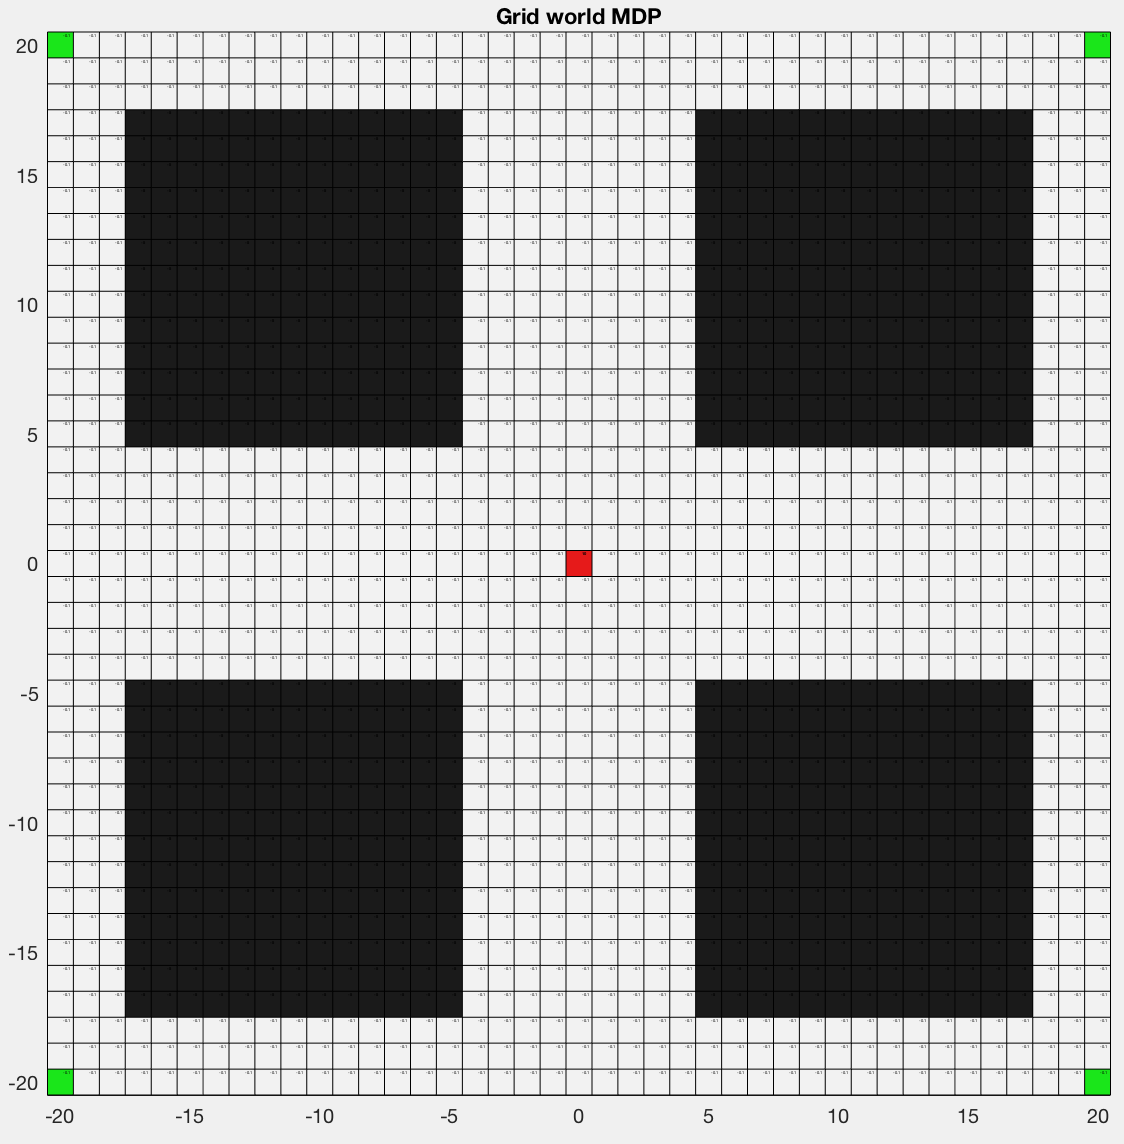
\includegraphics[width=0.65\linewidth]{maze_grid}
			\end{center}
		}
		
		\frame[t]
		{
			$\blacksquare$ Optimal Policy (value iteration) : 
			\vspace{-5pt}
			\begin{center}
				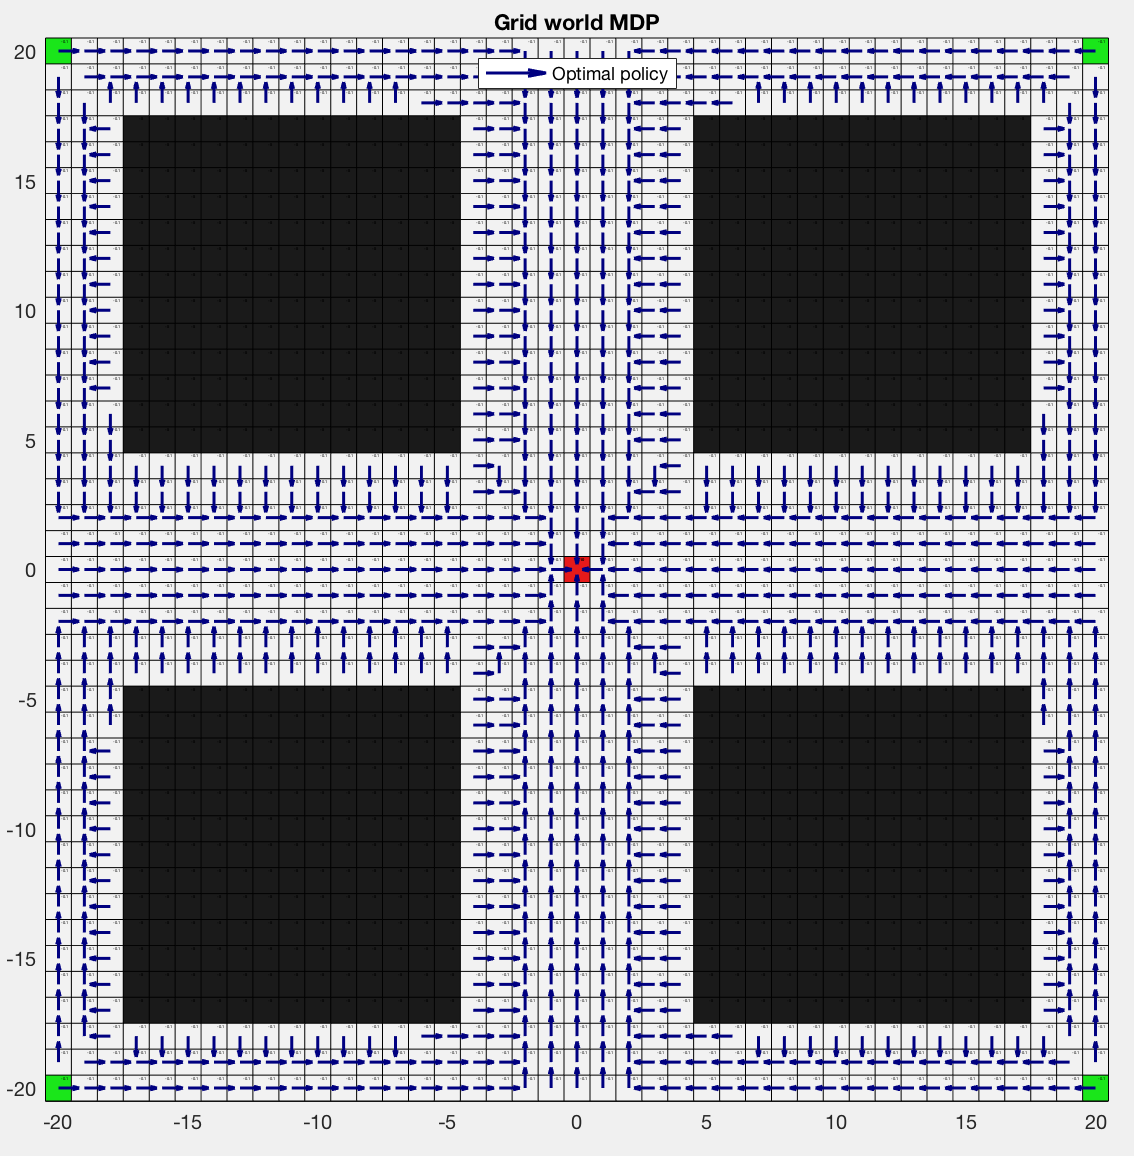
\includegraphics[width=0.65\linewidth]{maze_optimal_policy}
			\end{center}
		}
		
		\frame[t]
		{
			$\blacksquare$ Learning the optimal policy
			\vspace{-5pt}
			\begin{center}
				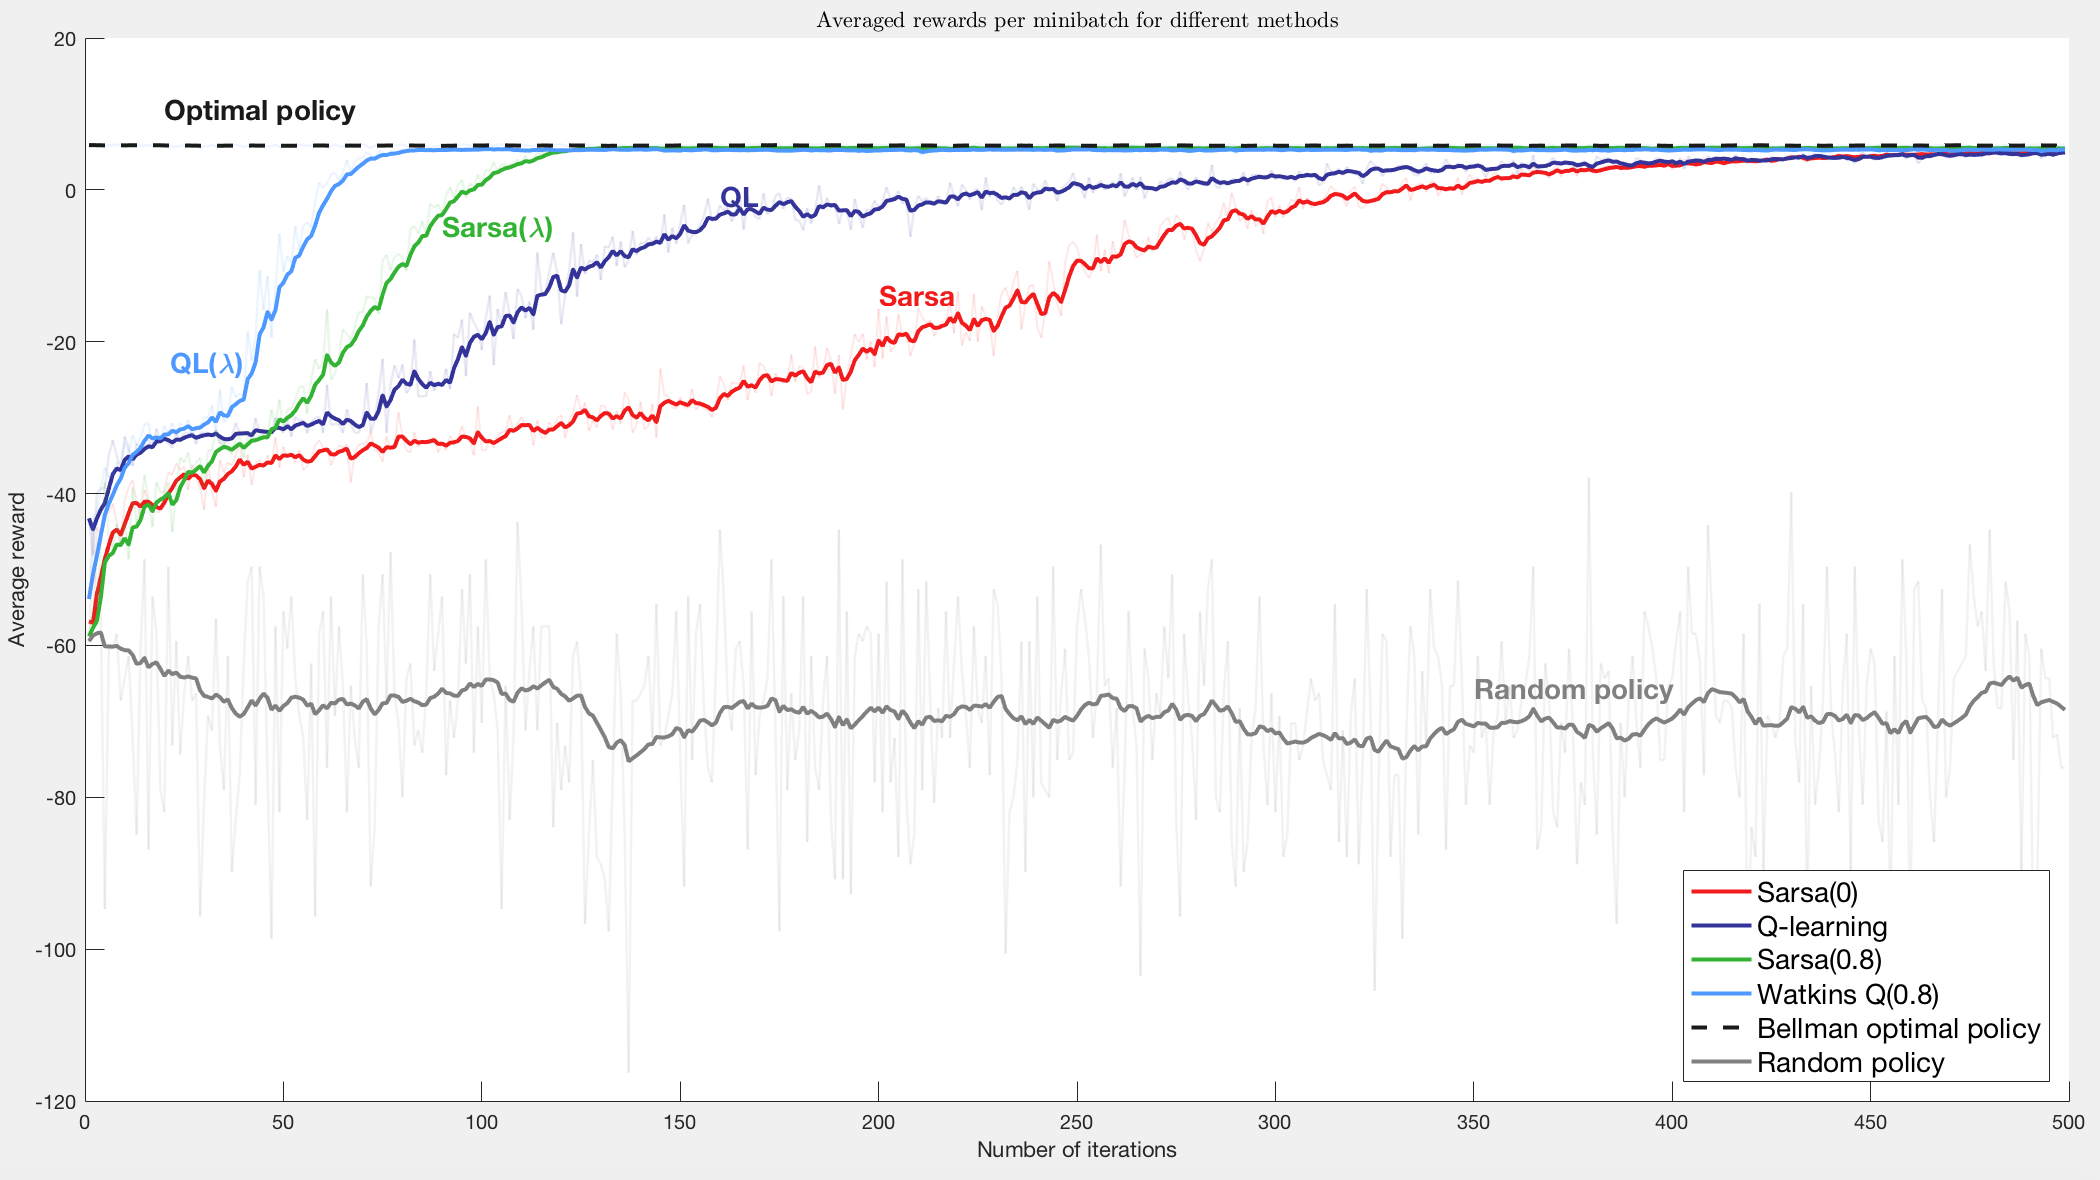
\includegraphics[width=\linewidth]{fullcompt_with_leg}
			\end{center}
		}
		\frame[t]
		{
			$\blacksquare$ Generating a suboptimal mentor 
			\vspace{-5pt}
			\begin{center}
				\begin{tikzpicture}
				 	 \node (img1) {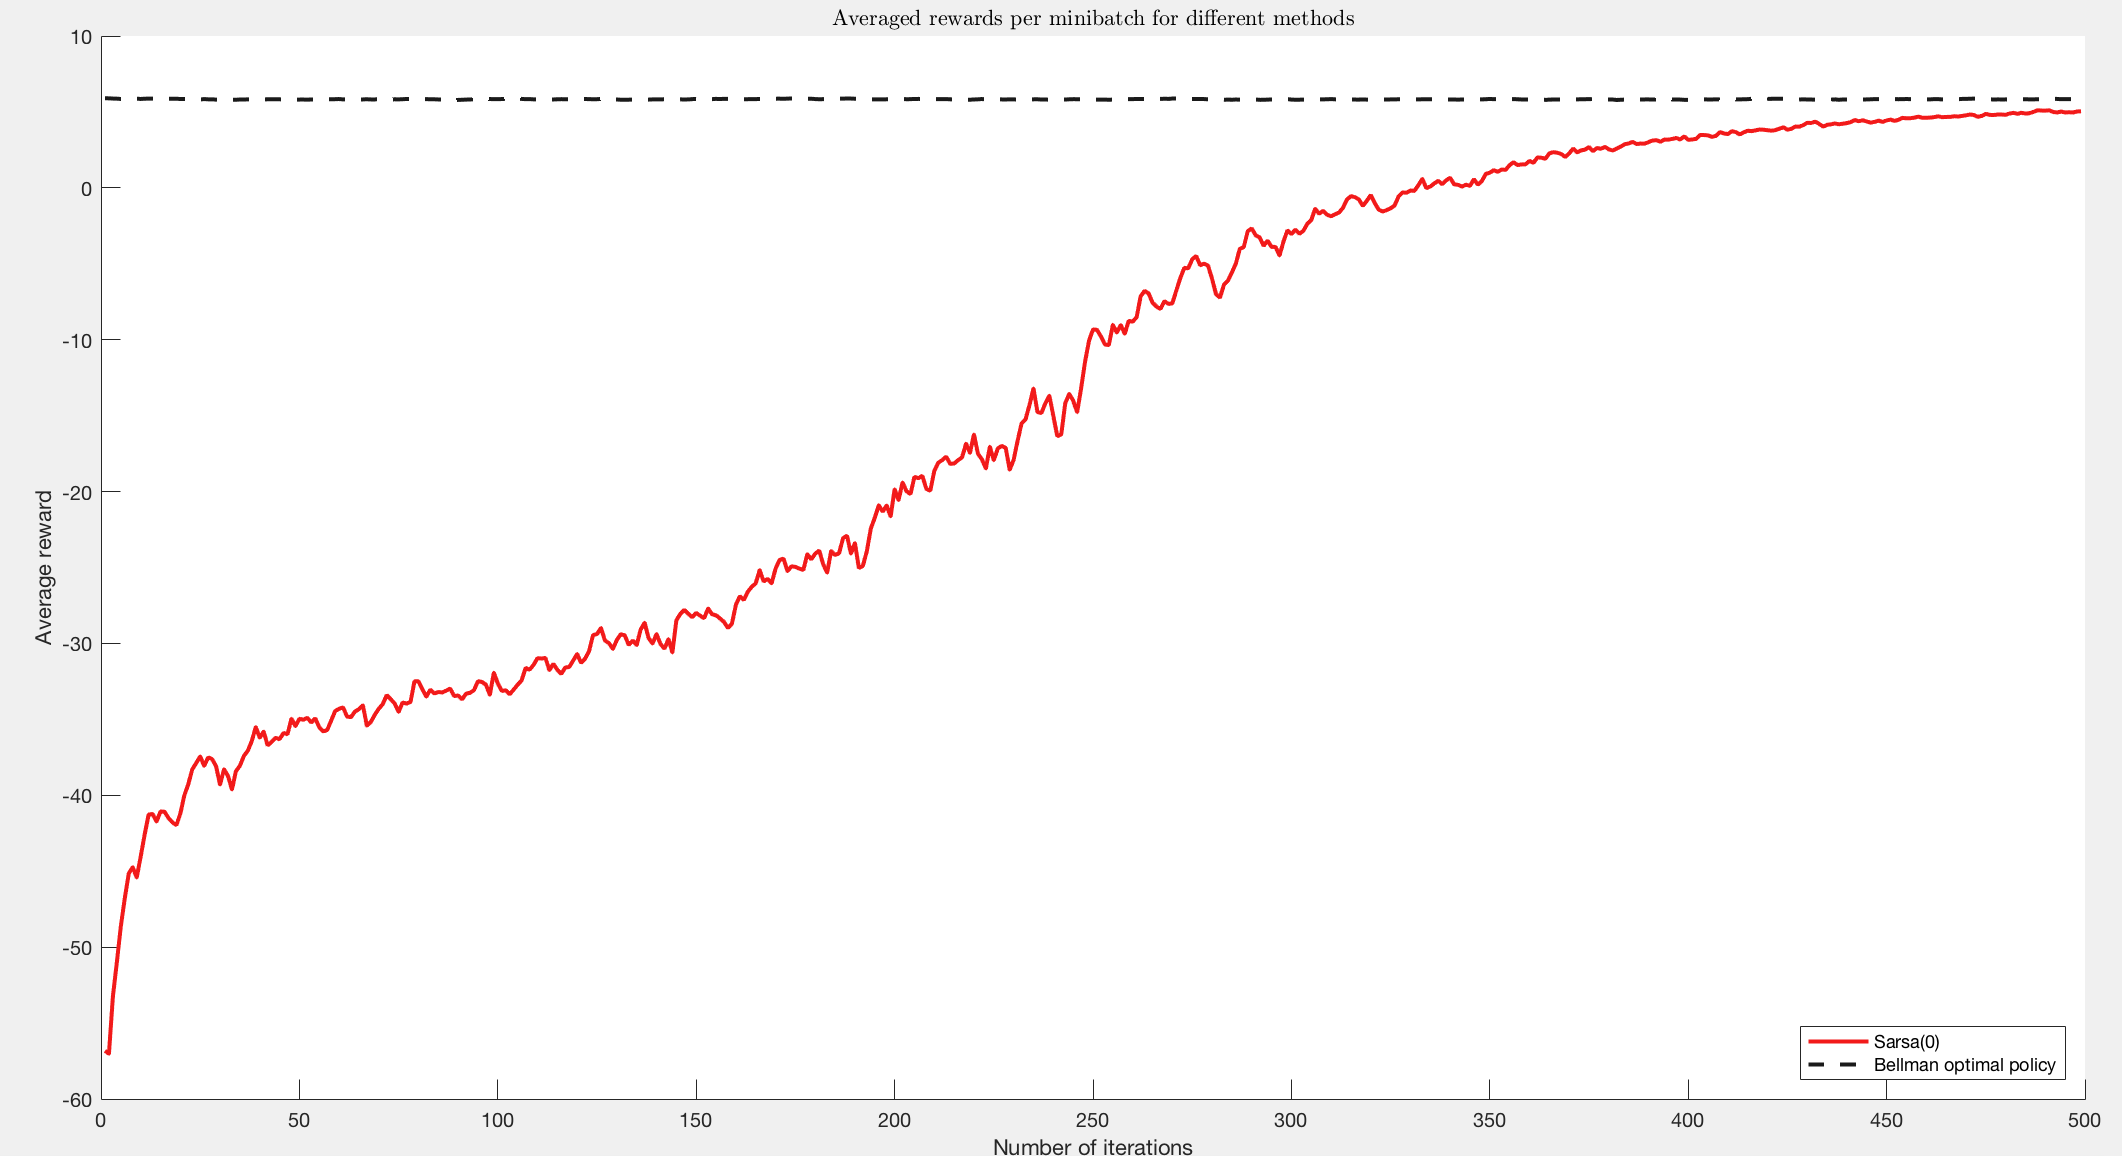
\includegraphics[width=\linewidth]{gen_mentor_1}};
 					 \pause
					  \node (img2) at (img1){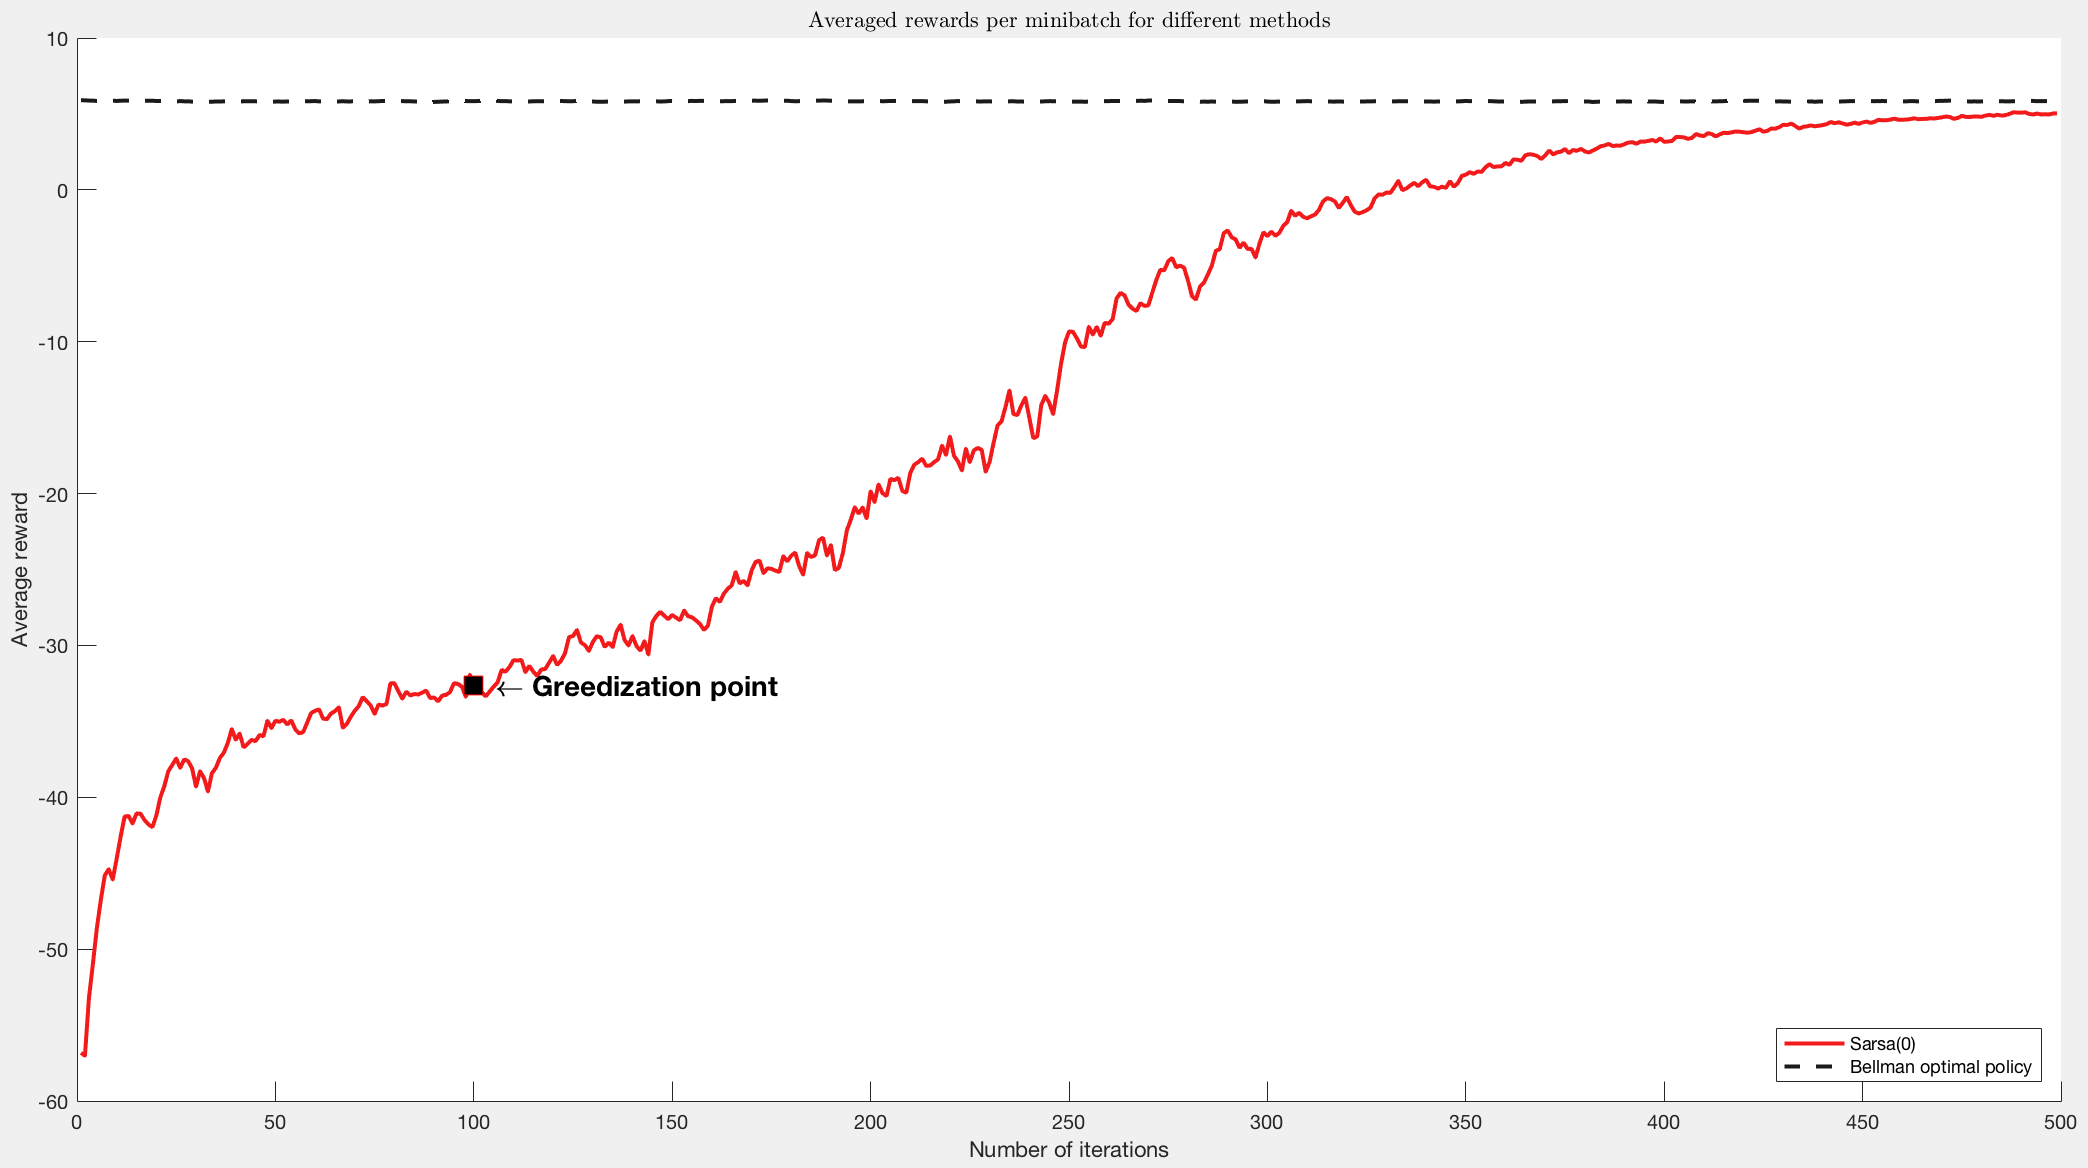
\includegraphics[width=\linewidth]{gen_mentor_2}};
					  \pause
 					 \node (img3) at (img1){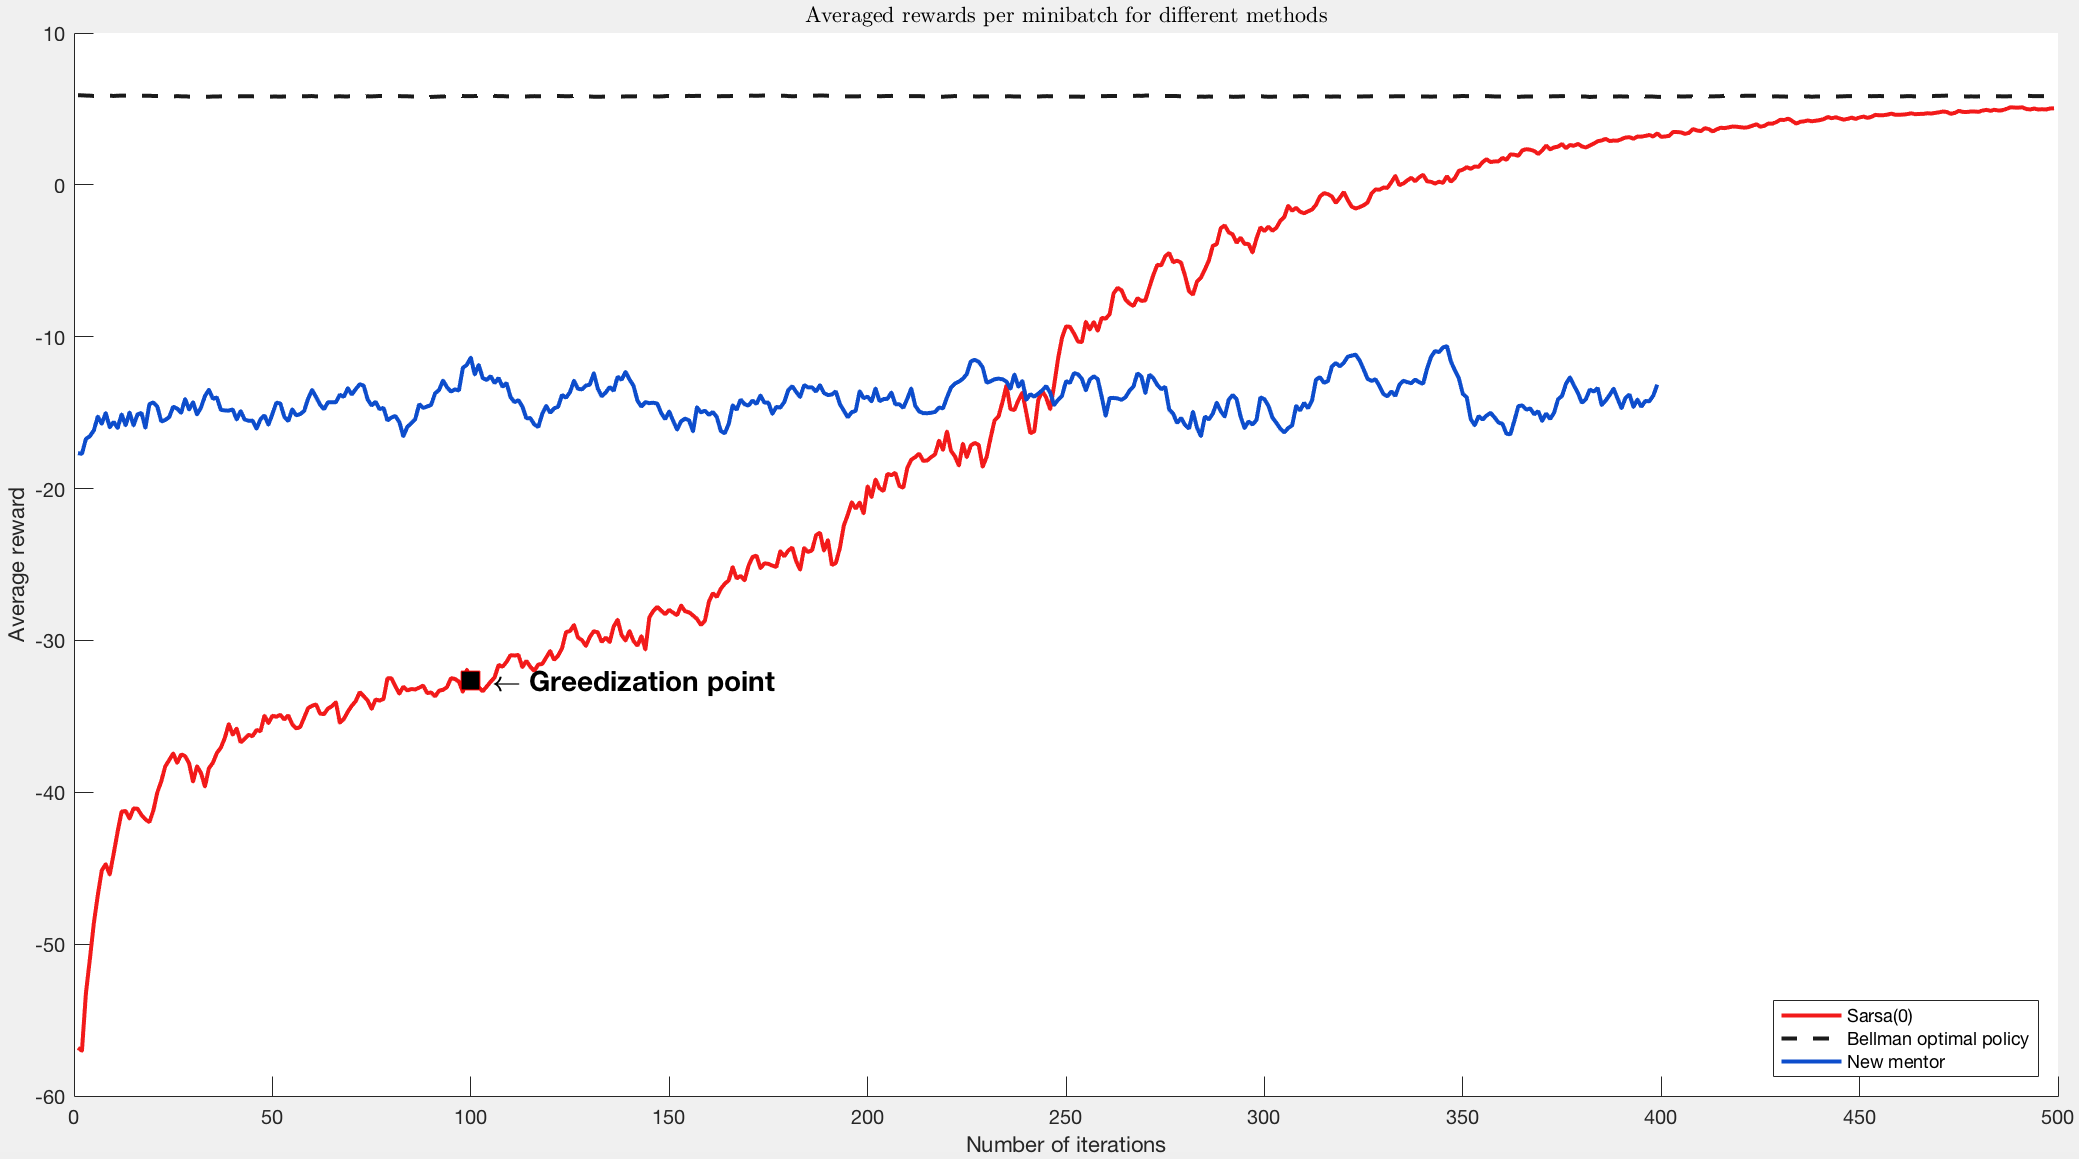
\includegraphics[width=\linewidth]{gen_mentor_3}};
				\end{tikzpicture}
			\end{center}
		}
	}
	\subsection{Compliance-based learning}
	{
		\frame[t]
		{
			\vspace{10pt}
			$\blacksquare$ Compliance learning 
			
			\vspace{10pt}
			$\color{red}\rightarrow$ Intuitively : 
				\begin{itemize}
					\item<sub@1> Follow the teacher 
					\item<sub@1> Gain some knowledge about the environment and the task 
					\item<sub@1> Take our own actions 
				\end{itemize} 
			\vspace{15pt}
			
			$\color{red}\rightarrow$ The teacher should only influence our action selection: 
			
			\begin{itemize}
			\item Global \textbf{compliance term} : $p\in[0,1]$
				\item $p$-greedy action selection w.r.t the mentor's action $a_m$ : $\forall s \in\mathcal{S}$
				\begin{equation}
					\pi(s) = \left\{
					\begin{aligned}
						&a_m \, \text{with probability }p \\
						& a \in \mathcal{A}(s) \text{ (Gibbs softmax)}
					\end{aligned}\right.
				\end{equation}
			\end{itemize}

		}
		
		\frame[t]
		{
			$\blacksquare$ \textcolor{red}{Vanishing compliance} : 
			\vspace{20pt}
			\begin{itemize}
				\item \textbf{Constantly decreasing compliance} : 
				\begin{equation}
				\left|
					\begin{aligned}
						&p_0 \in [0,1]\\
						&p_{t+1} = \beta p_t, \quad \beta < 1
					\end{aligned}\right.
				\end{equation}
				\item Along with SARSA update : 
				\begin{equation}
					Q(s,a) \leftarrow Q(s,a) + \alpha(r + \gamma Q(s',a') - Q(s,a))
				\end{equation}
			\end{itemize}
			\vspace{20pt}
			
			$\color{red}\blacktriangleright$ Start with $p_0\simeq 1$ (high confidence) and slowly decide to take your own decisions. 
		}
		
		\frame[t]
		{
			$\blacksquare$ Constantly decreasing compliance : 
			\vspace{10pt}
			\begin{figure}[h!]
				\begin{center}
					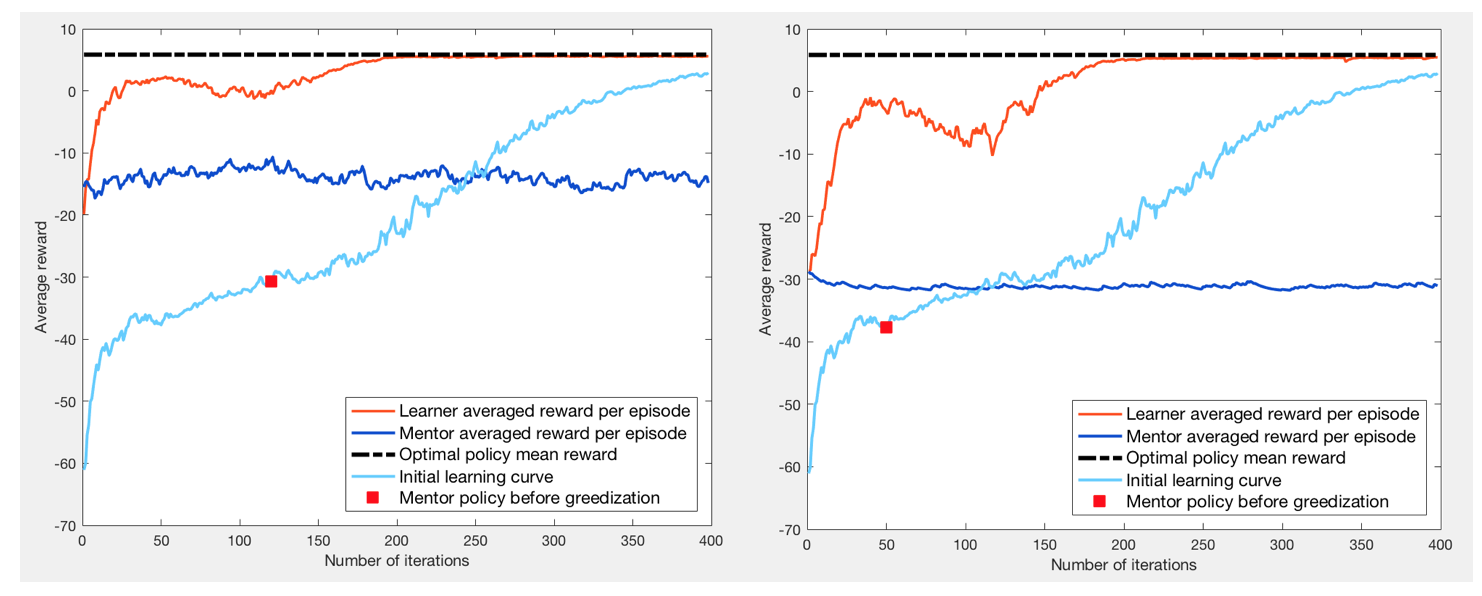
\includegraphics[width=\linewidth]{naive_comp}
					\caption{Average reward for two naive compliance learners}
				\end{center}
			\end{figure}
		}
		
		\frame[t]
		{
			\vspace{20pt}
			$\blacksquare$ Learning the compliance term\\ 
			\vspace{10pt}
			$\forall s\in\mathcal{S}$, define $p(s)$ - compliance term that impact the action selection : 
			\begin{equation}
				\pi(s) = \left\{
				\begin{aligned}
					&a_m \, \text{with probability }p(s)\\
					& a \in \mathcal{A}(s)\backslash a_m  \text{ with probabiliy 1-p(s)}
				\end{aligned}\right.
			\end{equation}
			
			\vspace{20pt}
			\textbf{Goal} : learn $p(s),\, \forall s \in\mathcal{S}$ $\rightarrow$ measure how right the teacher seems to be 
		}
		\frame[t]
		{
			$\color{red}\blacktriangleright$	\textbf{Implicit $\beta$-compliance} : 
			\vspace{5pt}
			\begin{itemize}
				\item $\forall s\in\mathcal{S}$, provide $p(s)$ with a Beta prior ($\alpha >> \beta$) 
					\begin{equation}
						p(s) \sim B (\alpha(s), \beta(s))
					\end{equation}
				\item Given a (s,a,r,s',a') 5-tuple, compute the critic TD value : 
				\begin{equation}
					\delta_t = r + \gamma Q(s',a') - Q(s,a_m) \quad \color{red} \rightarrow\text{\small{\textcolor{red}{how good is the teacher ?}} }	\color{black}	
				\end{equation}
				\item Compute \textbf{posterior distribution} over $p(s)$ :
				\begin{equation}
				\label{eq::update_rule}
				\begin{aligned}
					\alpha_t(s) &\leftarrow \alpha_t(s) +  \mathds{1}_{a=a_m}\delta_t \eps_t\\
					\beta_t(s) &\leftarrow \beta_t(s) +   \mathds{1}_{a\neq a_m}\delta_t\eps_t
				\end{aligned}
			\end{equation}
			\end{itemize}
		}
		
		\frame[t]
		{
			$\color{red}\blacktriangleright$	\textbf{Implicit $\beta$-compliance} :  
			\begin{figure}[h!]
				\begin{center}
					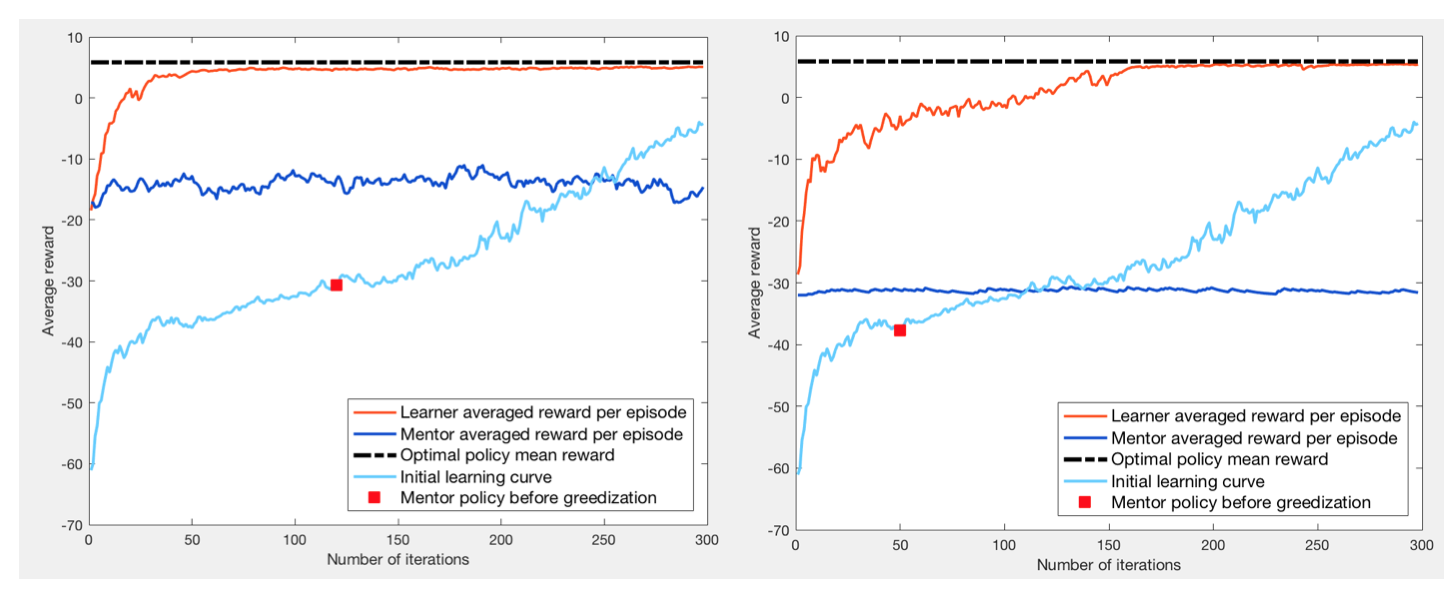
\includegraphics[width=\linewidth]{ac_comp}
					\caption{Average reward for two actor-critic compliance learners}
				\end{center}
			\end{figure}
			\begin{itemize}
				\item Faster convergence 
				\item No undershoot + tuning is intuitive  
			\end{itemize}
		}
		
		\frame[t]
		{
			$\color{red}\blacktriangleright$ \textbf{Implicit $\beta$-compliance} : 
			\begin{figure}[h!]
				\begin{center}
					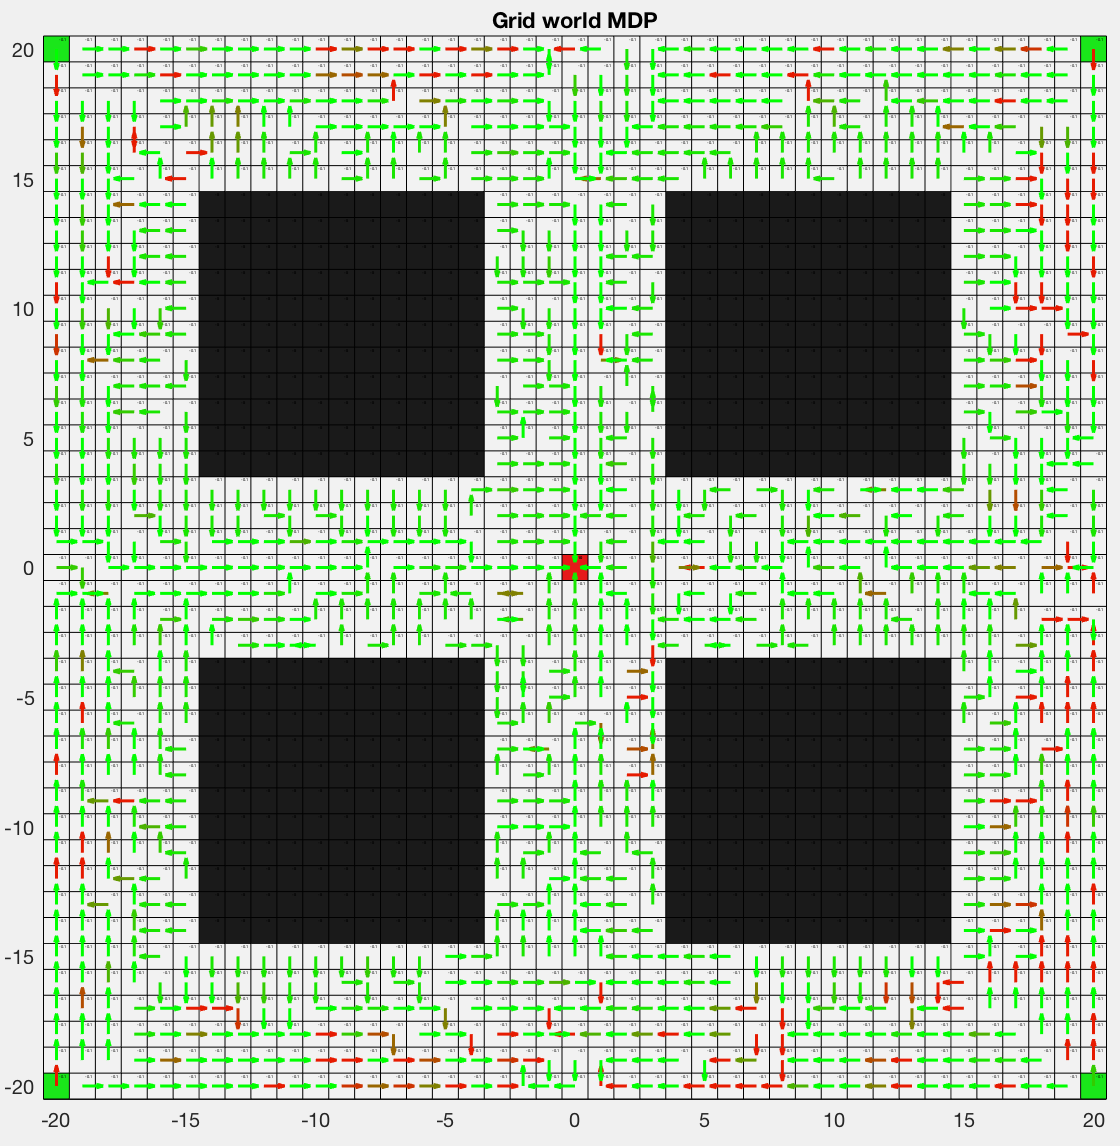
\includegraphics[width=0.6\linewidth]{heatmap_confidence_120}
					\caption{Posterior mean of $p$}
				\end{center}
			\end{figure}
		}
		
		\frame[t]
		{
			$\color{red}\blacktriangleright$	\textbf{Explicit compliance} : 
			\begin{itemize}
				\item Adds a hierarchical MDP : 
				\begin{equation}
					\forall s\in\mathcal{S}, \, \mathcal{A}_c(s) = \left\{ 'listen', \, 'discard'\right\}
				\end{equation}
				\item Define exploration based on $\{Q_c(s,l), Q_c(s,d)\}$ : 
				\begin{equation}
				\forall s \in\mathcal{S}, \quad \pi_c(s) = 
					\left\{
						\begin{aligned}
							&'l' \text{ with probability } p(s)=\sigma\left(\frac{Q_c(s,l) - Q_c(s,d)}{\tau} \right) \\
							& 'd'  \text{ with probability } 1-p(s)
						\end{aligned}
					\right.
			\end{equation}
			\item Perform SARSA update 
				\item Update : 
				\begin{equation}
					\left\{
					\begin{aligned}
						&Q_c(s,l) \leftarrow  \beta Q_c(s,l) + (1-\beta)Q(s,a_m) \\
						&Q_c(s,d) = \beta Q_c(s,d) + (1-\beta)\max_{a\neq a_m} Q(s,a) 
					\end{aligned}
					\right.
				\end{equation}

			\end{itemize}
		}
		
		\frame[t]
		{
			$\color{red}\blacktriangleright$	\textbf{Explicit compliance} : 
			\begin{figure}[h!]
				\begin{center}
					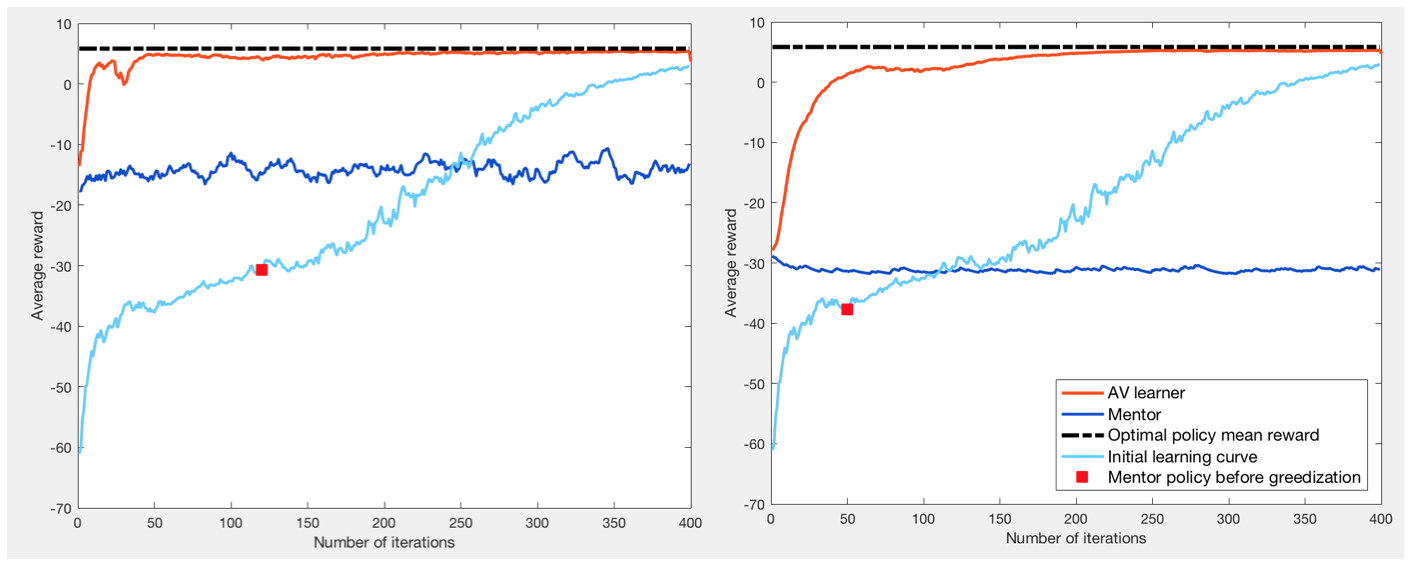
\includegraphics[width=\linewidth]{av_comp}
					\caption{Average reward for two action-value compliance learners}
				\end{center}
			\end{figure}

		}
		\frame[t]
		{
			$\color{red}\blacktriangleright$	\textbf{Explicit compliance} :
			\begin{figure}[h!]
				\begin{center}
					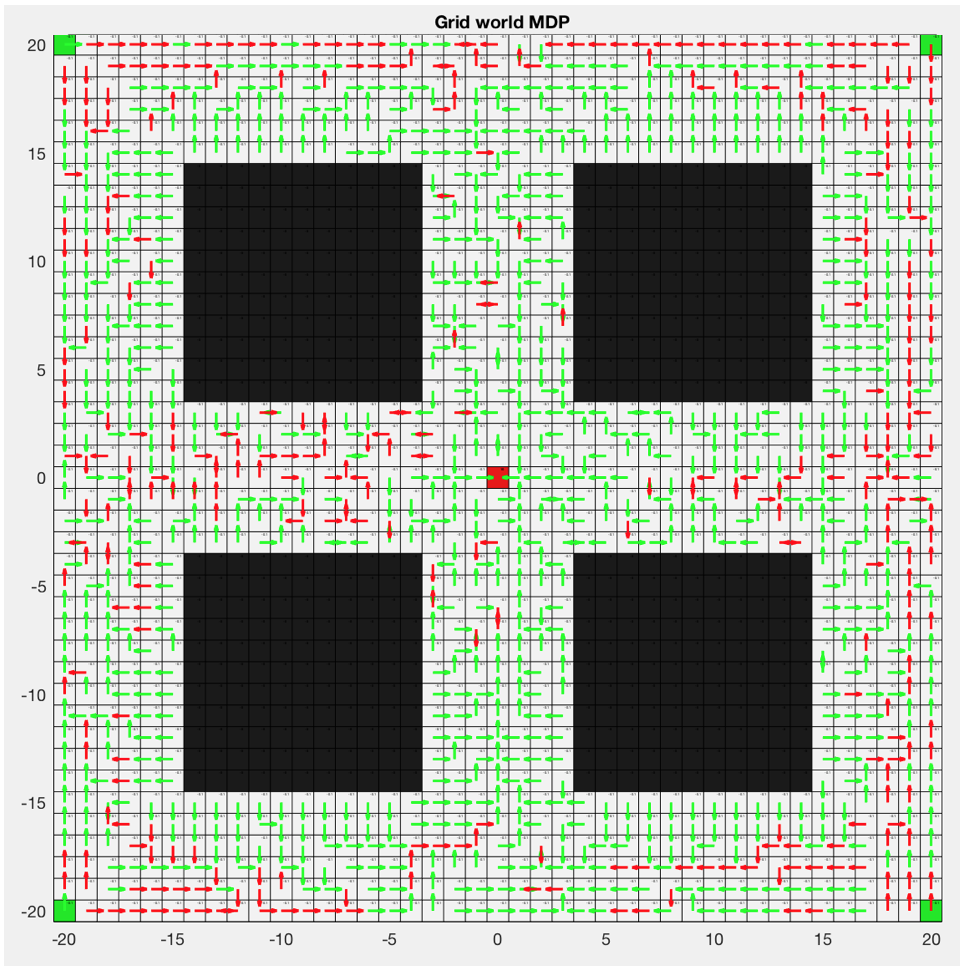
\includegraphics[width=0.6\linewidth]{heatmap_decision_50}
					\caption{Posterior decisions}
				\end{center}
			\end{figure}
		}
	}
	\subsection{Method comparaison}
	{
	
		\frame[t]
		{
			$\color{red}\blacktriangleright$	\textbf{Method comparaison} : learning curves 
			\vspace{-10pt}
			\begin{center}
				 \begin{tikzpicture}
				 	 \node (img1) {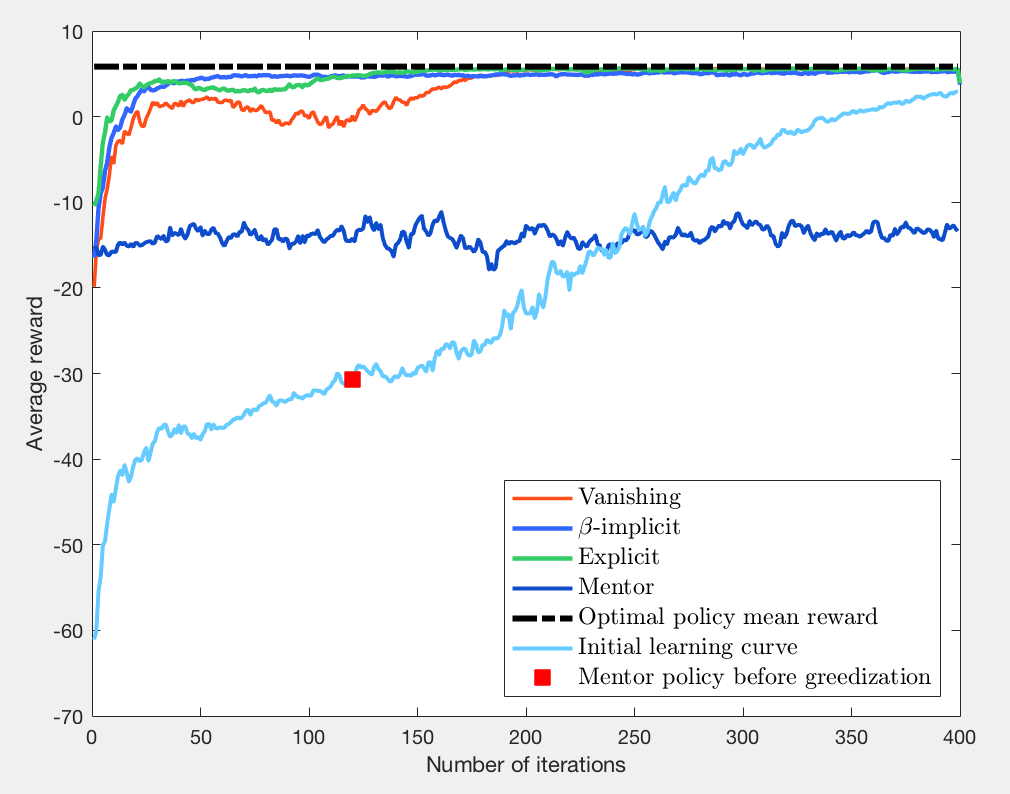
\includegraphics[width=0.8\linewidth]{fullcomp_subopt_120}};
 					 \pause
					  \node (img2) at (img1){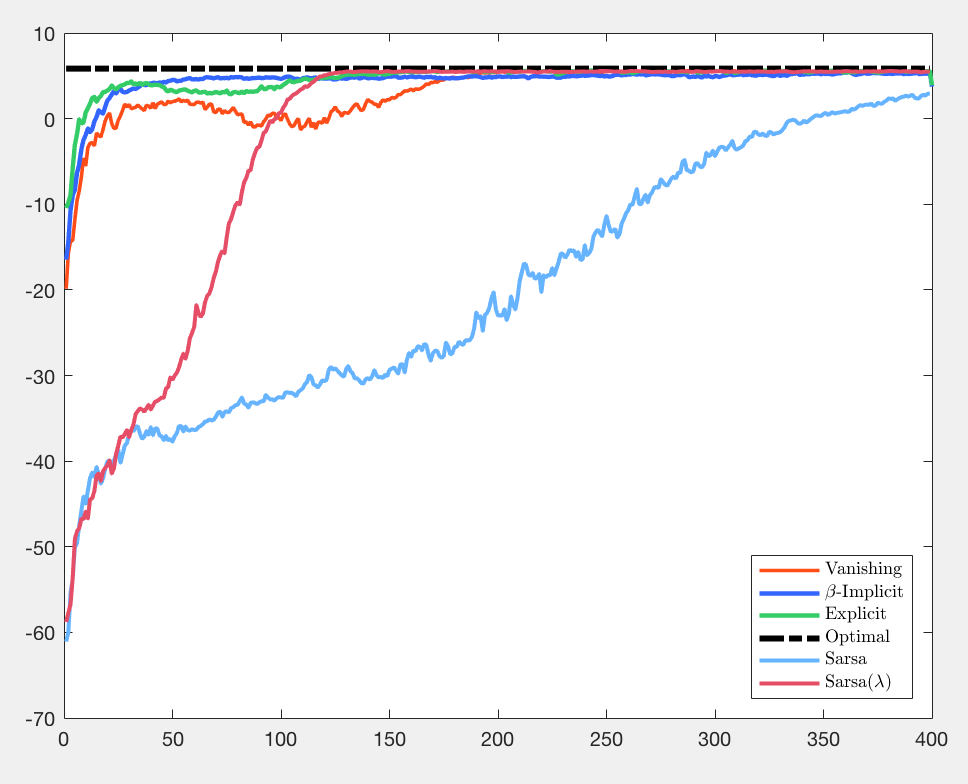
\includegraphics[width=0.8\linewidth]{fullcomp_subopt_120_w_loners}};
					  \pause
					  \node (img3) at (img1){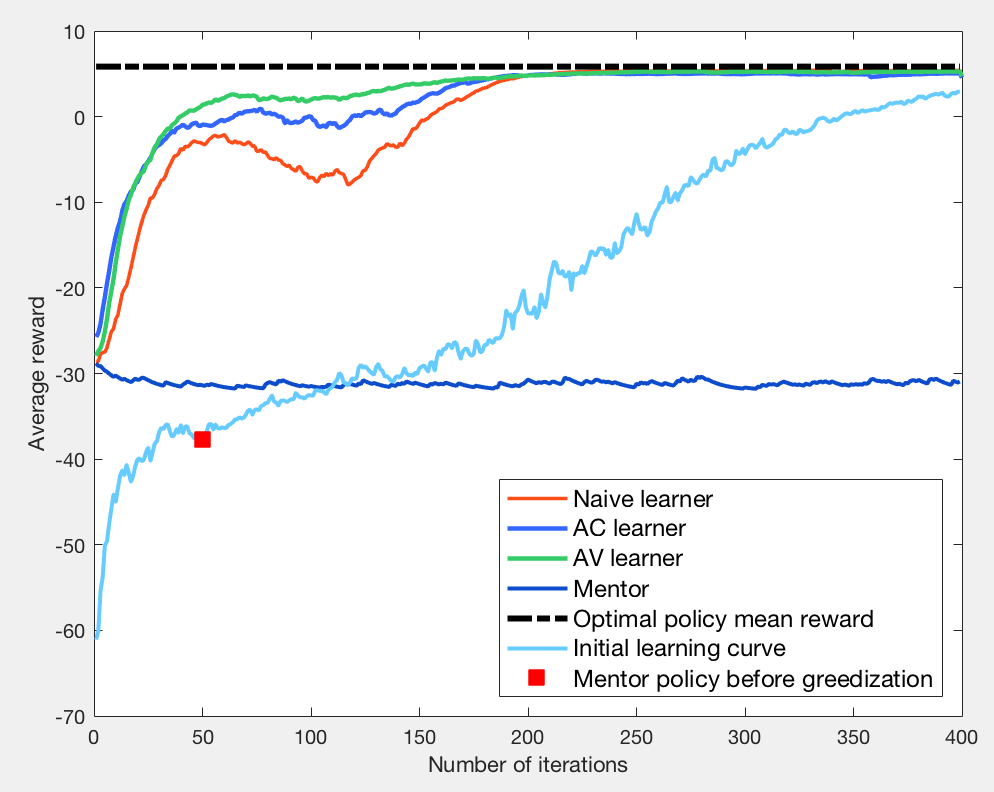
\includegraphics[width=0.8\linewidth]{fullcomp_subopt_50}};
				\end{tikzpicture}
			\end{center}
		}
		
		\frame[t]
		{
			$\color{red}\blacktriangleright$	\textbf{Method comparaison} : f-fold metrics statistics 
			\vspace{20pt}
			\begin{center}
				 \begin{figure}
				 	\begin{minipage}{\linewidth}
				 	 	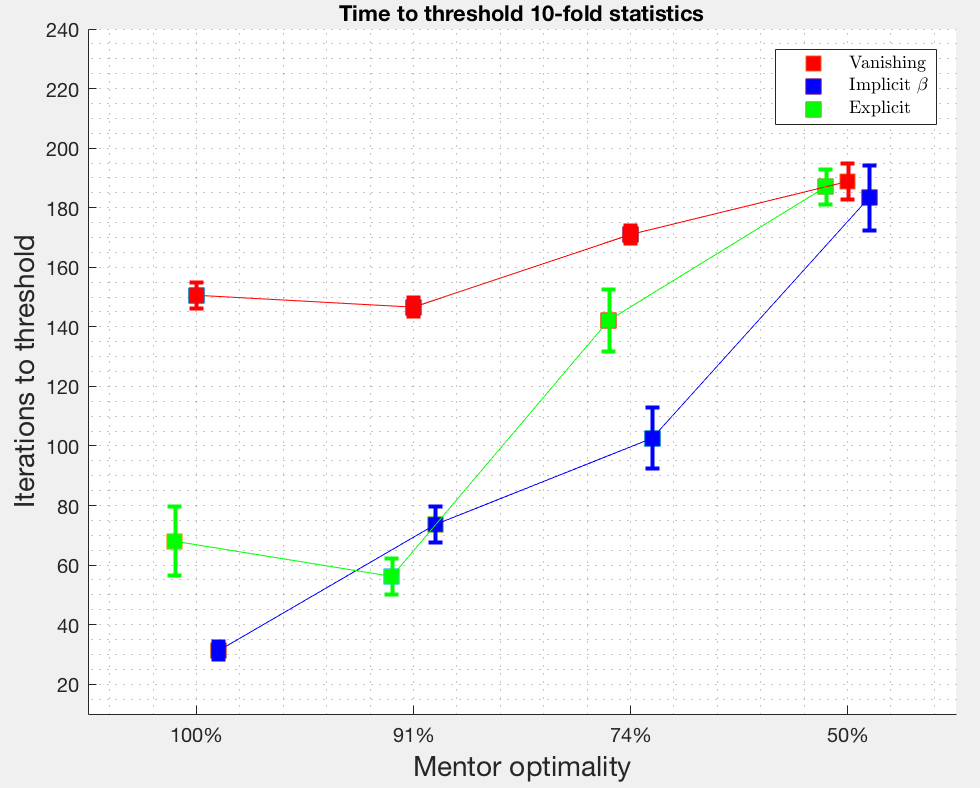
\includegraphics[width=0.5\linewidth]{tt_metric}
 					 \pause
					  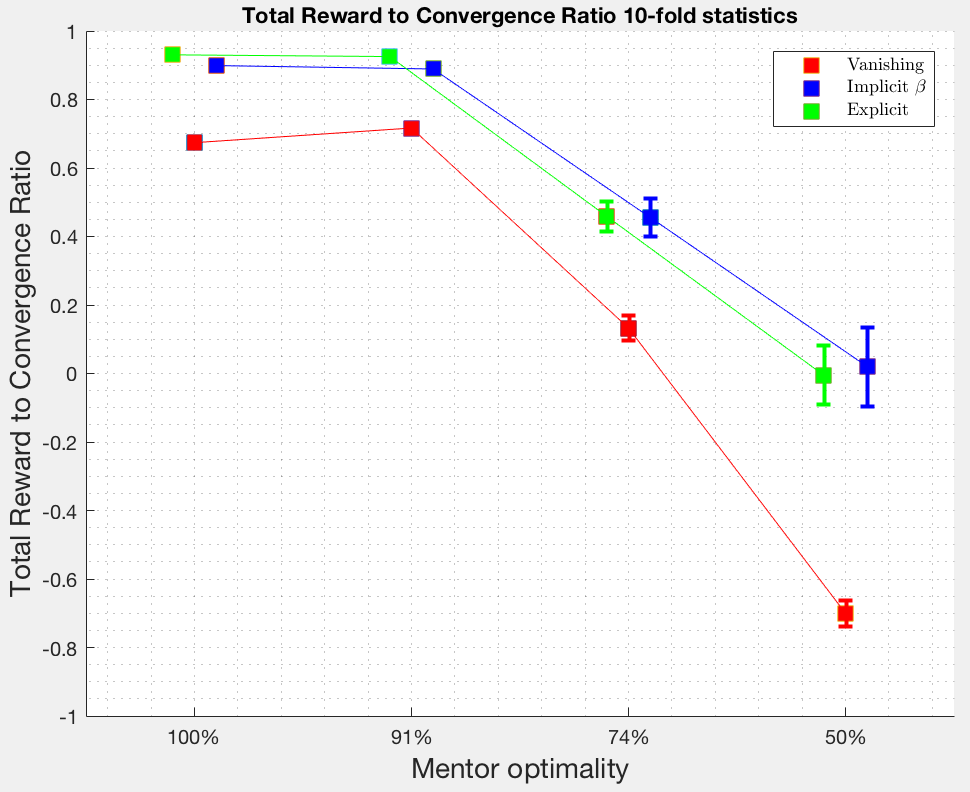
\includegraphics[width=0.49\linewidth]{tr_metric}
					\end{minipage}
				\end{figure}
			\end{center}
		}
	}
}

\section{Future work}
{
	\begin{frame}[t]
		$\color{red}\blacktriangleright$	\textbf{Future Work}
		\vspace{20pt}
		\begin{itemize}
			\setlength\itemsep{2em}
			\item Convergence and final result is too much impacted by the mentor : \textbf{off-policy} generalization 
			\item Eligibility-trace formulation 
			\item Generalize to several mentors 
			\item Generalize to sparse recommandations 
		\end{itemize} 
	\end{frame}
}

\frame[t]
{
	\vspace{70pt}
	\begin{center}
		\textbf{\huge{\textcolor{red}{Thank you for your attention !}}}
	\end{center}
}

\end{document}